
  
\documentclass[journal,12pt,twocolumn]{IEEEtran}

\usepackage{setspace}
\usepackage{gensymb}
\singlespacing
\usepackage[cmex10]{amsmath}

\usepackage{amsthm}

\usepackage{mathrsfs}
\usepackage{txfonts}
\usepackage{stfloats}
\usepackage{bm}
\usepackage{cite}
\usepackage{cases}
\usepackage{subfig}

\usepackage{longtable}
\usepackage{multirow}

\usepackage{enumitem}
\usepackage{mathtools}
\usepackage{steinmetz}
\usepackage{tikz}
\usepackage{circuitikz}
\usepackage{verbatim}
\usepackage{tfrupee}
\usepackage[breaklinks=true]{hyperref}
\usepackage{graphicx}
\usepackage{tkz-euclide}

\usetikzlibrary{calc,math}
\usepackage{listings}
    \usepackage{color}                                            %%
    \usepackage{array}                                            %%
    \usepackage{longtable}                                        %%
    \usepackage{calc}                                             %%
    \usepackage{multirow}                                         %%
    \usepackage{hhline}                                           %%
    \usepackage{ifthen}                                           %%
    \usepackage{lscape}     
\usepackage{multicol}
\usepackage{chngcntr}

\DeclareMathOperator*{\Res}{Res}

\renewcommand\thesection{\arabic{section}}
\renewcommand\thesubsection{\thesection.\arabic{subsection}}
\renewcommand\thesubsubsection{\thesubsection.\arabic{subsubsection}}

\renewcommand\thesectiondis{\arabic{section}}
\renewcommand\thesubsectiondis{\thesectiondis.\arabic{subsection}}
\renewcommand\thesubsubsectiondis{\thesubsectiondis.\arabic{subsubsection}}


\hyphenation{op-tical net-works semi-conduc-tor}
\def\inputGnumericTable{}                                 %%

\lstset{
%language=C,
frame=single, 
breaklines=true,
columns=fullflexible
}
\begin{document}

\newcommand{\BEQA}{\begin{eqnarray}}
\newcommand{\EEQA}{\end{eqnarray}}
\newcommand{\define}{\stackrel{\triangle}{=}}
\bibliographystyle{IEEEtran}
\raggedbottom
\setlength{\parindent}{0pt}
\providecommand{\mbf}{\mathbf}
\providecommand{\pr}[1]{\ensuremath{\Pr\left(#1\right)}}
\providecommand{\qfunc}[1]{\ensuremath{Q\left(#1\right)}}
\providecommand{\sbrak}[1]{\ensuremath{{}\left[#1\right]}}
\providecommand{\lsbrak}[1]{\ensuremath{{}\left[#1\right.}}
\providecommand{\rsbrak}[1]{\ensuremath{{}\left.#1\right]}}
\providecommand{\brak}[1]{\ensuremath{\left(#1\right)}}
\providecommand{\lbrak}[1]{\ensuremath{\left(#1\right.}}
\providecommand{\rbrak}[1]{\ensuremath{\left.#1\right)}}
\providecommand{\cbrak}[1]{\ensuremath{\left\{#1\right\}}}
\providecommand{\lcbrak}[1]{\ensuremath{\left\{#1\right.}}
\providecommand{\rcbrak}[1]{\ensuremath{\left.#1\right\}}}
\theoremstyle{remark}
\newtheorem{rem}{Remark}
\newcommand{\sgn}{\mathop{\mathrm{sgn}}}
\providecommand{\abs}[1]{\vert#1\vert}
\providecommand{\res}[1]{\Res\displaylimits_{#1}} 
\providecommand{\norm}[1]{\lVert#1\rVert}
%\providecommand{\norm}[1]{\lVert#1\rVert}
\providecommand{\mtx}[1]{\mathbf{#1}}
\providecommand{\mean}[1]{E[ #1 ]}
\providecommand{\fourier}{\overset{\mathcal{F}}{ \rightleftharpoons}}
%\providecommand{\hilbert}{\overset{\mathcal{H}}{ \rightleftharpoons}}
\providecommand{\system}{\overset{\mathcal{H}}{ \longleftrightarrow}}
	%\newcommand{\solution}[2]{\textbf{Solution:}{#1}}
\newcommand{\solution}{\noindent \textbf{Solution: }}
\newcommand{\cosec}{\,\text{cosec}\,}
\providecommand{\dec}[2]{\ensuremath{\overset{#1}{\underset{#2}{\gtrless}}}}
\newcommand{\myvec}[1]{\ensuremath{\begin{pmatrix}#1\end{pmatrix}}}
\newcommand{\mydet}[1]{\ensuremath{\begin{vmatrix}#1\end{vmatrix}}}
\numberwithin{equation}{subsection}
\makeatletter
\@addtoreset{figure}{problem}
\makeatother
\let\StandardTheFigure\thefigure
\let\vec\mathbf
\renewcommand{\thefigure}{\theproblem}
\def\putbox#1#2#3{\makebox[0in][l]{\makebox[#1][l]{}\raisebox{\baselineskip}[0in][0in]{\raisebox{#2}[0in][0in]{#3}}}}
     \def\rightbox#1{\makebox[0in][r]{#1}}
     \def\centbox#1{\makebox[0in]{#1}}
     \def\topbox#1{\raisebox{-\baselineskip}[0in][0in]{#1}}
     \def\midbox#1{\raisebox{-0.5\baselineskip}[0in][0in]{#1}}
\vspace{3cm}
\title{Assignment 5}
\author{Adarsh Sai - AI20BTECH11001}
\maketitle
\newpage
\bigskip
\renewcommand{\thefigure}{\theenumi}
\renewcommand{\thetable}{\theenumi}
Download all python codes from 
\begin{lstlisting}
https://github.com/Adarsh541/AI1103-prob-and-ranvar/blob/main/Assignment5/codes/Assignment5.py
\end{lstlisting}

%
Download latex-tikz codes from 
%
\begin{lstlisting}
https://github.com/Adarsh541/AI1103-prob-and-ranvar/blob/main/Assignment5/Assignment5.tex
\end{lstlisting}
\section{Problem(GATE 2020(ST) Q16)}
The characteristic function of a random variable X is given by
\begin{align}
\phi_{X}\brak{t}
=
\begin{cases}
\frac{\sin{t}\cos{t}}{t}           & t \neq 0 \\
1        & t = 0
\end{cases}
\end{align}
Then $ P\brak{|X|\leq \frac{3}{2}} =$ 
\section{Solution(GATE 2020(ST) Q16)}
The pdf is given by
\begin{align}
    f_{X}(x) = \frac{1}{2\pi} \int_{-\infty}^{\infty}  \phi_{X}\brak{t}e^{-jxt} dt 
\end{align}
If
\begin{align}
    g\brak{x} &\system{F} G\brak{t}\\
    \implies G\brak{t} &\system{F} g\brak{-x} \label{th}
\end{align}
where $ \brak{\system{F}}$ represents Fourier transform and
\begin{align}
    G\brak{t}  = \int_{-\infty}^{\infty} g\brak{x} e^{-j2\pi xt} dx 
\end{align}
we know that the Fourier transform of rectangular function is sinc function
\begin{align}
    rect\brak{\frac{x}{\tau}} &\system{F} \tau sinc(t\tau)
\end{align}
from \eqref{th} we get
\begin{align}
  \tau sinc(t\tau) &\system{F} rect\brak{-\frac{x}{\tau}}
\end{align}
\begin{align}
 \implies rect\brak{-\frac{x}{\tau}} = \int_{-\infty}^{\infty} \tau \frac{\sin{\pi t \tau}}{{\pi t \tau}} e^{-j2\pi xt}dt
\end{align}
substituting $\tau = \frac{2}{\pi}$ and changing $2\pi x \rightarrow x $ we get
\begin{align}
    \frac{1}{4}rect\brak{\frac{-x}{4}} = \frac{1}{2\pi} \int_{-\infty}^{\infty} \brak {\frac{\sin{2t}}{2t}}e^{-jxt} dt 
\end{align}
So
\begin{align}
    f_{X}(x) &= \frac{1}{4}rect\brak{\frac{-x}{4}}\\
    P\brak{|X|\leq \frac{3}{2}} &= \int_{\frac{-3}{2}}^{\frac{3}{2}} \frac{1}{4} dx\\
    &=\frac{3}{4}
\end{align}
\begin{figure}[!ht]
\centering
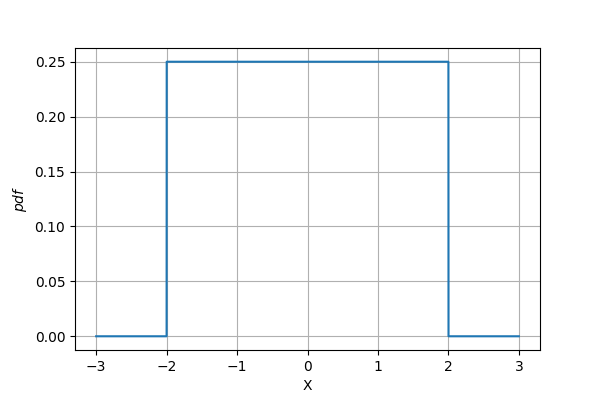
\includegraphics[width=\columnwidth]{Assignment5.png}
\caption{$f_{X}(x)$}
\label{pdf}
\end{figure}
\end{document}

